
\chapter{Fundamentação Teórica}\label{cap:fundamentacao}

Neste capítulo serão aprofundados os principais fundamentos que formam a base teórica na qual foi firmado o presente trabalho, dentre estes: representações intermediárias de código, forma de atribuição única estática, ANF e o \emph{framework} LLVM.

\section{Representações Intermediárias de Código}

A compilação de um programa é feita por meio de diversas etapas, entre as quais são necessárias representações que permitam a comunicação, ou que facilitem certos processamentos, como otimizações, análises e a geração de código. Segundo \citeonline{dragao}, ao traduzir um programa da linguagem fonte para código de máquina de uma arquitetura específica, o compilador cria uma série de representações intermediárias (IRs).

Existem diversos modelos de IRs de código, cada um com suas aplicações específicas em diferentes etapas do processo de compilação. Por exemplo, as árvores sintáticas abstratas são usualmente construídas durante a análise sintática de um programa, e podem ser utilizadas também durante a geração do código de saída. Grafos de Fluxo de Controle (CFG - \emph{Control Flow Graph}) são usados em fases analíticas e auxiliam, por exemplo, na identificação de código inatingível nos programas, nesse caso possibilitando otimizações do artefato final a ser gerado.

\begin{figure}[htpb]
    \centering
    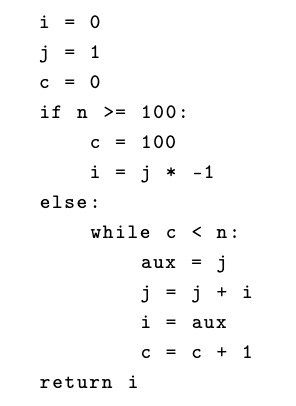
\includegraphics[width=0.3\textwidth]{Imagens/codigo-ex.jpg}
    \caption{Se $n >= 100$ retorna -1, senão retorna o n-ésimo número de Fibonacci}
    \label{fig:ex-codigo}
    \small{Fonte: O autor}
\end{figure}

% \begin{figure}[htpb]
% \lstset{%
%     caption=Exemplo de código que calcula o primeiro número de fibonatti maior que n,
%     basicstyle=\ttfamily\footnotesize\bfseries,
%     xleftmargin=.35\textwidth,
% }\label{list:ex-codigo}
% \begin{lstlisting}[language=Python]
% i = 0
% j = 1
% c = 0
% if n >= 100:
%     c = 100
%     i = j * -1
% else:
%     while c < n:
%         aux = j
%         j = j + i
%         i = aux
%         c = c + 1
% return i
% \end{lstlisting}
% \end{figure}

Na Figura \ref{fig:cfg-example1} é apresentado um exemplo de representação intermediária na forma de um Grafo de Fluxo de Controle referente ao código que calcula o número de Fibonacci presente da Figura \ref{fig:ex-codigo}. Nessa IR o código é representado por um grafo no qual cada nó contém um bloco de expressões sequenciais e novos nós e arestas são adicionados quando existem condicionais ou \emph{gotos} (vá para), expressando os diferentes caminhos possíveis de execução por meio de um grafo. Nessa representação intermediária os caminhos de execução no fluxos de controle do programa são evidenciados.

\begin{figure}
    \centering
    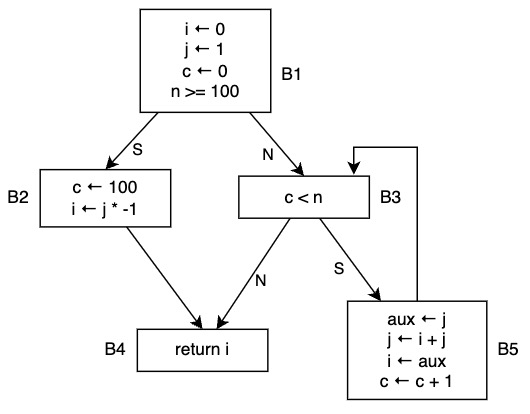
\includegraphics[width=0.6\textwidth]{Imagens/cfg-ex5.jpg}
    \caption{Exemplo de Grafo de IR em Fluxo de Controle da Figura \ref{fig:ex-codigo}}
    \label{fig:cfg-example1}
    \small{Fonte: O autor}
\end{figure}

Ao demonstrar os usos das IRs durante o processo de tradução de código, \citeonline{dragao} classifica-as em duas categorias, de acordo com seu uso ao longo da transformação do código fonte para código de máquina:

\begin{itemize}
\item \textbf{Representações Intermediárias de Alto Nível}: Estão mais próximas da linguagem fonte e são utilizadas nas primeiras etapas da tradução do código. Exemplos incluem as árvores sintáticas abstratas, que descrevem a estrutura direta do código fonte e são úteis em tarefas como a checagem estática de tipos.
\item \textbf{Representações Intermediárias de Baixo Nível}: Aproximam-se mais da máquina alvo e aparecem em etapas posteriores da tradução do código fonte. Focam em tarefas específicas da máquina alvo, como alocação de registradores e seleção de instruções.
\end{itemize}

Além dos usos já citados, com o advento das novas propostas de projeto de compiladores modulares e reutilizáveis, as IRs têm desempenhado um papel importante ao permitir a comunicação do \emph{frontend}, que é encarregado de fazer a leitura e tratamentos do código fonte, com o \emph{backend} que, por sua vez, faz otimizações, análises e pode gerar como saída o código de máquina para a arquitetura alvo. Nesse caso de uso a IR serve como uma linguagem para a comunicação entre as interfaces dos diferentes componentes do compilador \cite{lattner2004llvm}. 

A Figura \ref{fig:llvm-ri-ex1} apresenta um exemplo de IR especificada e usada pela LLVM, código que imprime no terminal a frase "Hello World!". Neste exemplo é possível observar que a representação intermediária gerada contém, além das definições e expressões necessárias, algum metadado que possivelmente será útil para as etapas seguintes da compilação. Na Seção \ref{sec:llvm-ir} a LLVM-IR será detalhada com mais profundidade.

\begin{figure}
    \centering
    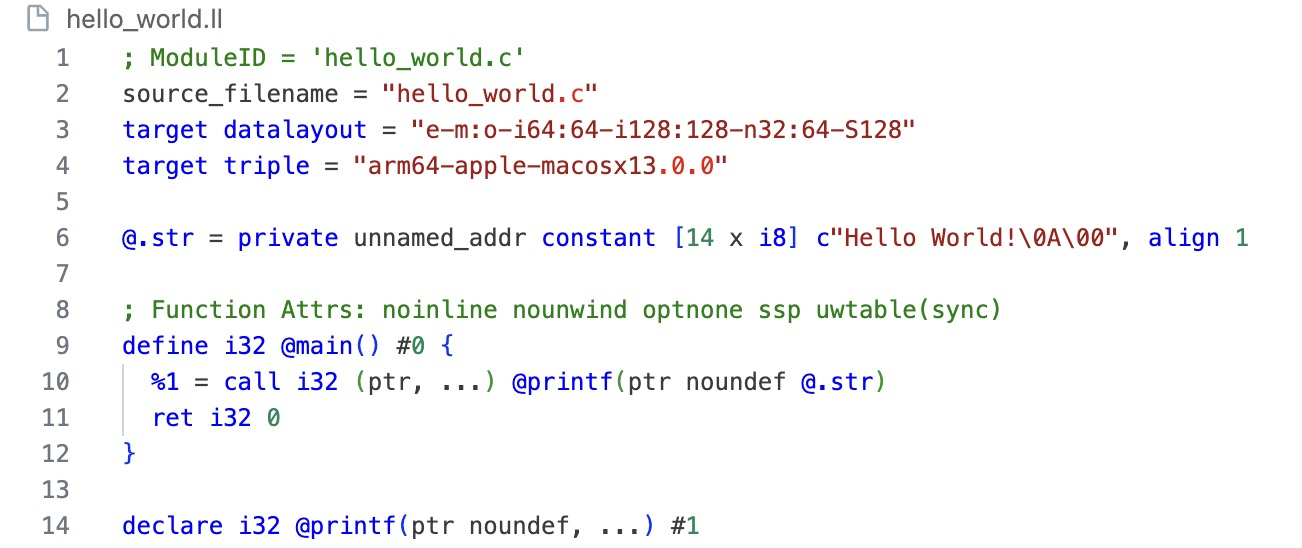
\includegraphics[width=0.8\textwidth]{Imagens/llvm-ir-ex1.jpg}
    \caption{Exemplo de IR em LLVM-IR}
    \label{fig:llvm-ri-ex1}
    \small{Fonte: O autor, gerado através do \emph{clang}}
\end{figure}

Ademais, é importante pontuar que, como visto nos exemplos, IRs podem ser tanto estruturas de dados armazenadas durante a execução do compilador, quanto uma linguagem em si, e seu uso vai depender de como o compilador foi projetado \cite{dragao}. Há inclusive a possibilidade de usar uma linguagem de programação como IR, por exemplo C, que compila para código nativo eficiente.

\section{Forma de Atribuição Única Estática}

É vastamente referenciado na literatura que a forma de atribuição única estática (SSA - \emph{Static Single-Assignment}) é de importante valor ao facilitar certas otimizações de código para linguagens imperativas \cite{appel1998ssa} \cite{dragao} \cite{muchnick1997advanced}. Sendo assim, utilizada de maneira ampla na implementação das etapas de otimização de código de compiladores e ferramentas de otimização de código, como é o caso da LLVM e do GCC (GNU Compiler Collection). % \cite{lattner2004llvm} https://pastel.hal.science/pastel-00002281/

Mais especificamente, \citeonline{muchnick1997advanced} traz alguns exemplos de algoritmos de otimização que SSA facilita e torna mais eficazes, principalmente referentes à análise do fluxo de dados de programas, como: propagação de constantes, numeração de valores, movimentação e remoção código invariante e remoção de redundância parcial. Segundo \citeonline{muchnick1997advanced}, isso segue do fato que na forma SSA há a separação dos valores contidos no programa, com base no lugar em que estes são usados.

Um procedimento está em forma de atribuição única estática quando cada variável que recebe um valor dentro dele é alvo de apenas uma atribuição \cite{muchnick1997advanced}. Ao passo que a cada atribuição uma nova variável deve ser criada, e dessa forma, as variáveis são imutáveis. Além disso, é definida a notação conceitual da função $\phi$, usada para unir definições de variáveis em caminhos divergentes no fluxo de controle, selecionando aquela pela qual o fluxo de controle passou durante a execução \cite{dragao}. Nota-se que a atribuição de uma variável pode ocorrer dentro de um laço de repetição, o que levaria a múltiplas definições desta, e iria contrariar as restrições da forma SSA. No entanto, a forma de atribuição única em SSA é uma característica estática do programa, e não uma propriedade dinâmica da execução \cite{appel1998ssa}. A Figura \ref{fig:not-ssa-vs-ssa} contém um exemplo de código e sua representação e ao lado sua representação em forma SSA, demonstrando a criação de novas variáveis a cada atribuição feita.

\begin{figure}[h]
\centering
\begin{subfigure}{.5\textwidth}
    \centering
    $$\displaylines{
    p \ \leftarrow \ a \ + \ b \cr
    q \ \leftarrow \ p \ - \ c \cr
    p \ \leftarrow \ p \ * \ q \cr
    p \ \leftarrow \ d \ - \ p \cr
    q \ \leftarrow \ p \ + \ q \cr
    }$$
    \caption{Não SSA}
    \label{fig:sub1}
\end{subfigure}%
\begin{subfigure}{.5\textwidth}
    \centering
    $$\displaylines{
    p_1 \ \leftarrow \ a \ + \ b \cr
    q_1 \ \leftarrow \ p_1 \ - \ c \cr
    p_2 \ \leftarrow \ p_1 \ * \ q_1 \cr
    p_3 \ \leftarrow \ d \ - \ p_2 \cr
    q_2 \ \leftarrow \ p_3 \ + \ q_1 \cr
    }$$
    \caption{Em forma SSA}
    \label{fig:sub2}
\end{subfigure}
\caption{Comparação entre atribuições em não SSA e em SSA}
\label{fig:not-ssa-vs-ssa}
\small{Fonte: O autor, adaptado de \citeonline{dragao}}
\end{figure}

O mecanismo padrão de tradução para a forma SSA é adicionar uma subscrição a cada variável toda vez que há uma atribuição, vide Figura \ref{fig:not-ssa-vs-ssa}, onde $p$ é dividido em $p_1$, $p_2$ e $p_3$ e $q$ se torna as duas variáveis $q_1$ e $q_2$. Porém, quando há mais de um caminho de execução em que uma mesma variável pode ser definida, há a necessidade de uma forma de unir estas. E é nesse momento que se faz o uso da função $\phi$, que tem a capacidade unir as definições divergentes de uma mesma variável nos pontos de junção do fluxo de controle.

A Figura \ref{fig:cfg-ssa-ex} contém um exemplo de como o programa da Figura \ref{fig:cfg-example1} fica na forma SSA. Nota-se o uso da função $\phi$ no ponto de junção para a variável $i$, o valor de $i_2$ naquele nó será atribuído ao valor do qual o fluxo de execução chega naquele bloco, podendo ter sido definida em B1 (onde é iniciado em 0) ou em B5 (recebendo o valor de aux$_1$).

\begin{figure}[h]
    \centering
    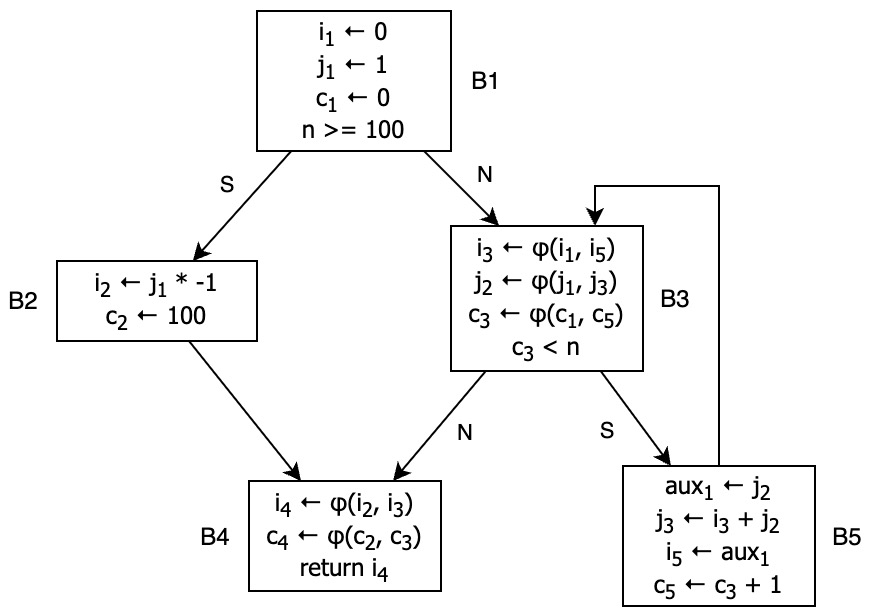
\includegraphics[width=0.6\textwidth]{Imagens/ssa-cfg-ex.jpg}
    \caption{CFG da Figura \ref{fig:cfg-example1} em forma SSA}
    \label{fig:cfg-ssa-ex}
    \small{Fonte: O autor}
\end{figure}

Há ainda o conceito de forma SSA mínima, que é a forma SSA que usa o menor número de funções $\phi$ possível. Para traduzir um código para a forma SSA mínima usa-se o conceito de fronteira de dominância (Definição \ref{def:dominance-frontier}) 
 \cite{cytron1991efficiently}.

É importante mencionar o uso de SSA na LLVM, um caso que demonstra a utilidade prática aplicada ao conjunto de ferramentas de compilação que está no estado da arte atualmente. Segundo \citeonline{lattner2004llvm}, a LLVM usa SSA como sua representação de código primária (exceto para definições de locação de memória), em que cada registrador virtual é escrito à exatamente uma instrução, e cada uso de registrador é dominado (Definição \ref{def:domination}) pela sua definição. \citeonline{lattner2004llvm} defendem o uso da forma SSA dizendo que esta oferece uma representação simplificada do fluxo de dados, facilitando muitas otimizações e possibilitando que algoritmos mais rápidos que não dependem do fluxo (\emph{flow-insensitive}) tirem proveito das vantagens de algoritmos que são sensíveis ao fluxo (\emph{flow-sensitive}), sem o custo de análises complexas no fluxo de dados. Adicionalmente, as mudanças que não envolvem \emph{loops} nessa estrutura são mais simples, já que não se deparam com dependências contrárias ou de saída em suas variáveis \cite{lattner2004llvm}.

\subsection{Árvore de Dominância} \label{sub:arvore-dominancia}

Conceitos advindos da teoria dos grafos como: dominância, fronteira de dominância, dominância imediata e árvore de dominância, são essenciais para este trabalho e são utilizados inclusive no método de tradução descrito no Capítulo \ref{cap:desenvolvimento}.

\begin{definition}[Dominação]\label{def:domination}
Na teoria de grafos, mais especificamente em grafos de fluxo, um nó $d$ é dito dominar um nó $n$ se, a partir do nó inicial, todos os caminhos até $n$ devem passar pelo nó $d$ \cite{muchnick1997advanced}. Notacionalmente $d \
dom \ n$. Nota-se que, por definição, todos os nós dominam si mesmos.
\end{definition}

\begin{definition}[Dominação Estrita]
Em um grafo de fluxo, um nó $d$ domina estritamente um nó $n$ se $d$ domina $n$ e $d \neq n$. Notacionalmente $d \ sdom \ n$.
\end{definition}

\begin{definition}[Predecessor e Predecessor Imediato]
Em um grafo de fluxo, um nó $n$ é predecessor de $m$ ($n \ pred \ m$) se existe pelo menos um caminho da origem até $m$ que passa por $n$; $n$ é considerado predecessor imediato ($Pred$) se em algum caminho é utilizada uma aresta de $m$ para $n$.
\end{definition}

\begin{definition}[Dominância Imediata]
O dominador imediato de um nó $n$ é o único nó que, domina estritamente $n$, mas não domina nenhum outro nó que domina estritamente $n$. Observa-se que todos os nós em um grafo de fluxo tem um dominador imediato, com exceção do inicial.
\end{definition}

\begin{definition}[Fronteira de Dominância]\label{def:dominance-frontier}
Sendo $x$ um nó do grafo de fluxo de controle, a fronteira de dominância de $x$ é o conjunto de todos os nós $y$ no grafo de fluxo tal que $x$ domina um predecessor imediato de $y$, mas não domina estritamente $y$ \cite{cytron1991efficiently}.
\end{definition}

Esses conceitos são principalmente utilizados ao analisar a dominância e dependência dos blocos dentro do grafo de fluxo de controle. Percebe-se que, se um bloco do grafo de fluxo de controle $n$ é dominado por outro nó $d$, as variáveis do bloco $d$ existem e podem ser acessadas no bloco $n$. Com isso, a estrutura de árvore de dominância favorece essa análise ao fornecer informação sobre o escopo das variáveis de um procedimento.

\begin{definition}[Árvore de Dominância]\label{def:dom-tree}
A árvore de dominância de um dado grafo de fluxo é a árvore em que os filhos de cada nó $n_i$ são os nós dominados imediatamente por $n_i$. A raiz da árvore é o nó inicial.
\end{definition}

A Figura \ref{fig:dominance-ex} contém um exemplo de árvore de dominância lado a lado ao grafo de fluxo de controle do código de exemplo da Figura \ref{fig:cfg-example1}. Percebe-se que o nó B4 é dominado somente pelo bloco B1 uma vez que há caminhos da origem até B4 que passam por B2 ou B3.

\begin{figure}
\centering
\begin{subfigure}{.5\textwidth}
  \centering
  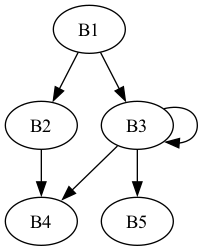
\includegraphics[width=.5\linewidth]{Imagens/graph-fig2.png}
  \caption{Grafo de fluxo de controle}
  \label{fig:sub1}
\end{subfigure}%
\begin{subfigure}{.5\textwidth}
  \centering
  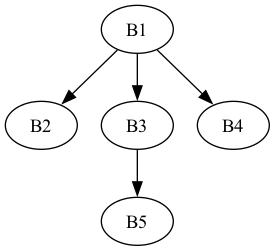
\includegraphics[width=.6\linewidth]{Imagens/dominance-fig2.png}
  \caption{Árvore de dominância}
  \label{fig:dom-tree}
\end{subfigure}
\caption{Comparação entre CFG e Árvore de Dominância do Código da Figura \ref{fig:cfg-example1}}
\label{fig:dominance-ex}
\small{Fonte: O autor}
\end{figure}

\section{ANF}

A Forma A-normal (ANF) é um conceito importante na compilação de programas funcionais, sendo utilizado frequentemente para simplificar a estrutura dos programas e facilitar otimizações. \citeonline{sabry1992reasoning} introduziram ANF como uma alternativa mais simples ao estilo de passagem de continuações (CPS, do inglês \emph{Continuation Passing Style}), demonstrando sua efetividade em transformações e otimizações de código funcional.

% \begin{figure}[h]
% \begin{center}
% \large
% \begin{tabular}{r@{\ \ }c@{\ \ }l}
%     $e$ & ::= & $v$ \ $|$ \ $e \ e$ \ $|$ \ $\lambda x. e$ \\
%     $v$ & ::= & $x$ \ $|$ \ $c$ \\
%     $x$ & $\in$ & \emph{variáveis} \\
%     $c$ & $\in$ & \emph{constantes} \\
% \end{tabular}
% \caption{Gramática Cálculo Lambda}
% \small{Fonte: O autor}
% \end{center}
% \label{fig:calculo-lambda}
% \end{figure}

% \igor{próximo parágrafo ta WIP}

% Em cálculo lambda puro, expressões podem ser: um valor, uma aplicação, ou uma abstração $\lambda$, vide a Figura \ref{fig:calculo-lambda}. Variáveis que não estão vinculadas a uma abstração $\lambda$ são ditas variáveis livres, o conjunto das variáveis livres de um termo $M$ é $FV(M)$. Em calculo lambda, é possível obter expressões como: $f \ (g \ 2) \ (h \ 3)$. Ao buscar por regras de redução para programas funcionais que pudessem prover um conjunto de axiomas no qual é possível provar que para dois termos $M$ e $N$, se $M = N$ então $CPS(M) = CPS(N)$. \citeonline{sabry1992reasoning} formularam as reduções vistas na Figura \ref{fig:reducoes} sobre a representação intermediária CPS. Após ter formulado tais regras, \citeonline{flanagan1993essence} descobrem o cálculo $\lambda_{\, v} \, A$, que não permite que tais reduções possam ser feitas, ou seja, o programa já está otimizado para as regras $\beta_{lift}$ e $\beta_{flat}$.

% \begin{figure}[h]
% \centering
% \begin{align*}
% ((\lambda x.M) \ V) & \rightarrow M[x := V] & & & & (\beta_v) \\
% (\lambda x.V x) & \rightarrow V & & x \notin FV(V) & & (\eta_v) \\
% E[((\lambda x.M) \ N)] & \rightarrow ((\lambda x.E[M]) \ N) & & x \notin FV(E) & & (\beta_{lift}) \\
% E[((M \ N) \ L)] & \rightarrow ((\lambda x.E[(x \ L)]) (M \ N)) & & x \notin FV(E, L) & & (\beta_{flat}) \\
% ((\lambda x.x) \ M) & \rightarrow M & & & & (\beta_d) \\
% ((\lambda x.E[(y \ x)]) \ M) & \rightarrow E[(y \ M)] & & x \notin FV(E[y]) & & (\beta_{\Omega})
% \end{align*}
% \caption{Reduções $A$ em CPS: $\{\eta_v, \beta_v, \beta_{lift}, \beta_{flat}, \beta_d, \beta_{\Omega}\}$}
% \label{fig:reducoes}
% \small{Fonte: \citeonline{sabry1992reasoning}}
% \end{figure}

Fundamentalmente, ANF é uma restrição a termos do cálculo-$\lambda$, na qual é imposto que os termos lambda sejam escritos em estilo direto \cite{ssaToAnf}. Em suma, isso quer dizer que os argumentos em aplicações de expressões devem ser termos atômicos (variáveis ou constantes). E que, para haver continuações na computação, são usadas variáveis temporárias atribuídas às sub-expressões do procedimento, e que são definidas em expressões \emph{let}. A Figura \ref{fig:llvm-ir-gramatica} apresenta um exemplo de gramática livre de contexto na qual não há como aninhar aplicações de expressões, sendo necessário que uma aplicação seja atribuída a uma variável antes de ser utilizada, ou seja, uma gramática na qual as produções são na forma ANF. Na notação utilizada, as classes gramaticais indicadas por uma linha superior (\emph{overline}) representam sequências de zero ou mais ocorrências dessas produções gramaticais. Pontua-se que ANF é definido conforme o cálculo-$\lambda$ com avaliação \emph{call-by-value} definido por \citeonline{plotkin1975call}.

\begin{figure}[h]
\begin{center}
\large
\begin{tabular}{r@{\ \ }c@{\ \ }l}
    $e$ & ::= & \textbf{let} \ $x$ \ \textbf{=} \ $v \ \overline{v}$ \ \textbf{in} \ $e$ \\
    & \ \ $|$ & $v \ \overline{v}$ \\
    $v$ & ::= & $x$ \ $|$ \ $c$ \ $|$ \ $\lambda x . e$ \\
    $x$ & $\in$ & \emph{variáveis} \\
    $c$ & $\in$ & \emph{constantes} \\
\end{tabular}
\caption{Gramática Exemplo de ANF}
\label{fig:llvm-ir-gramatica}
\small{Fonte: O autor}
\end{center}
\end{figure}

Em ANF o grafo de fluxo de controle é explícito, uma vez que chamadas de cauda são claramente distinguidas por sua posição dentro das expressões \emph{let}: chamadas de função no lado direito de uma atribuição de variável indicam chamadas normais, enquanto aquelas que aparecem no corpo significam chamadas de cauda, ou \emph{jumps} no fluxo de controle \cite{ssaToAnf}. Essa representação explícita de chamadas e chamadas de cauda simplifica análises sobre a execução do programa e facilita as otimizações nesse sentido. A Figura \ref{fig:lambda-vs-anf} apresenta um exemplo de como uma expressão fica quando escrita em ANF.

Semelhante à forma SSA, ANF codifica explicitamente o fluxo de dados ao nomear todas as sub-expressões dentro do programa e ao permitir apenas uma definição para cada variável \cite{ssaToAnf}. No entanto, ANF impõe essa restrição dinamicamente, pois um novo escopo é criado em tempo de execução para cada invocação de função. O escopo sintático claro em ANF facilita muitas otimizações que envolvem movimento de código entre blocos, o que pode ser mais complexo em SSA devido à necessidade de manter a propriedade de dominância entre a definição e uso das variáveis \cite{ssaToAnf}.

\begin{figure}[h]
\centering
\begin{subfigure}{.5\textwidth}
    \centering
    \begin{lstlisting}[language=Haskell,xleftmargin=.1\textwidth]
h (f (g x + 1)) (k (y * 2))
    \end{lstlisting}
    \caption{Não ANF}
    \label{fig:sub1}
\end{subfigure}%
\begin{subfigure}{.5\textwidth}
    \centering
    \begin{lstlisting}[language=Haskell,xleftmargin=.2\textwidth]
let a = g x in
let b = a + 1 in
let c = y * 2 in
let d = k c in
let e = f b in
h e d
    \end{lstlisting}
    \caption{Em ANF}
    \label{fig:sub2}
\end{subfigure}
\caption{Comparação de uma expressão em ANF}
\label{fig:lambda-vs-anf}
\small{Fonte: O autor}
\end{figure}

Dadas suas vantagens e aplicabilidade no paradigma funcional, variantes de ANF são usadas na prática como representação intermediária de diversos compiladores de linguagens funcionais, como GHC de Haskell \cite{jones1998transformation}, e TIL de ML \cite{wegman1991constant}. Ao usar ANF, estas ferramentas acrescentam algumas características como: permitir tuplas, funções com mais de um argumento, operações primitivas e condicionais. Na Seção \ref{sec:desenvolvimento-anf} é apresentada a gramática livre de contexto variante de ANF desenvolvida neste trabalho, e que é a saída do método de tradução desenvolvido.

\subsection{Tradução entre SSA e ANF}

Devido às características em comum de, por exemplo, não permitir mais de uma atribuição a uma mesma variável e ter o fluxo de controle explícito, pode-se inferir que existe uma relação entre a forma SSA e programação funcional. Mais do que isto, \citeonline{kelsey1995correspondence} e \citeonline{appel1998ssa} demonstraram que ambas são correspondentes, existindo um algoritmo que faz a tradução estática entre elas.

De maneira mais formal, \citeonline{ssaToAnf} definem um procedimento para a tradução de SSA para ANF, e demonstram que uma otimização, que é geralmente feita através de SSA, também pode ser feita utilizando ANF. O procedimento de \citeonline{ssaToAnf} servirá como base para a implementação deste trabalho apresentada no Capítulo \ref{cap:desenvolvimento}. Fazer a tradução de SSA para ANF envolve a construção da árvore de dominância (vista na Seção \ref{sub:arvore-dominancia}) sobre o grafo de fluxo de controle da forma SSA. A árvore serve como base para a construção dos escopos das funções em ANF. No código em ANF as funções correspondem tanto ao programa completo, quanto a estrutura do grafo de fluxo de controle de um procedimento específico \cite{ssaToAnf}. Os parâmetros das funções são determinados pelos $\phi$s do bloco de SSA, e o \emph{jumps} são traduzidos para chamadas de cauda.

\begin{figure}[h]
    \centering
\lstset{%
    xleftmargin=.17\textwidth,
}    
\begin{lstlisting}[language=Haskell,style=nasm]
fib n =
  let b1 () =
        let i1 = 0
            j1 = 1
            c1 = 0
            b2 () =
              let c2 = 100
                  i2 = j1 * (-1)
              in b4 i2 c2
            b3 i3 j2 c3 =
              let b5 () =
                    let aux1 = j2
                        j3 = i3 + j2
                        i5 = aux1
                        c5 = c3 + 1
                    in b3 i5 j3 c5
              in if c3 < n then b5 ()
                           else b4 i3 c3
            b4 i4 c4 = let in i4
        in if n >= 100 then b2 ()
                       else b3 i1 j1 c1          
    in b1 ()
\end{lstlisting}    
    \caption{Programa funcional em ANF em Haskell referente ao CFG da Figura \ref{fig:cfg-ssa-ex}}
    \label{fig:eq-ssa-func}
    \small{Fonte: O autor}
\end{figure}

A Figura \ref{fig:eq-ssa-func} contém um exemplo de código em ANF referente ao SSA da Figura \ref{fig:cfg-ssa-ex}. Nessa sintaxe, o ANF desse código é executável no GHC. Observa-se nesse exemplo que cada bloco é traduzido para uma função. Dentro do escopo dos blocos estão também as funções referentes aos blocos imediatamente dominados por estes. Os $\phi$s do bloco determinam seus argumentos, e para determinar o valor dos argumentos nas chamadas de função é necessário buscar o valor que seria atribuído pelo $\phi$ a partir do bloco que está fazendo a chamada.

No que se refere a este trabalho, \citeonline{rigon2020inferring} exploraram tal correspondência ao propor a definição do núcleo de uma linguagem puramente funcional, e a implementação de um algoritmo de inferência de tipos para código funcional que é gerado a partir de sua representação em forma SSA.

\section{LLVM}

O \emph{framework} LLVM (do inglês Máquina Virtual de Baixo Nível) foi projetado e desenvolvido com a proposta de oferecer um conjunto de ferramentas para análise e transformação de código arbitrário \cite{lattner2004llvm}. Este \emph{framework} vem se consolidando desde sua criação, e tornou-se uma parte fundamental no design de diversos compiladores modernos, sendo adotado por grandes empresas de tecnologia como Apple com o \emph{clang}, Google na plataforma Android e Mozilla com Rust. Isso se deve principalmente devido à sua capacidade de otimização de código, suporte a várias linguagens de programação e designs de hardware, e arquitetura modular que favorece o acoplamento de seus módulos em outros sistemas.

Segundo \citeonline{lattner2004llvm}, a LLVM tem dois principais pontos que a diferenciam das demais soluções, e que serão melhor explorados nessa seção: o projeto do compilador e a representação intermediária utilizada no \emph{framework}. Segundo \citeonline{lattner2004llvm}, o compilador é construído num modelo modular que é capaz de explorar a LLVM-IR como interface desses módulos, dessa forma fornecendo uma vasta combinação de capacidades quanto à otimização e tradução de código.

A Figura \ref{fig:llvm-design} apresenta uma visão de alto nível da arquitetura do sistema da LLVM e é explicada pelos autores como segue:

\begin{citacao}
Resumidamente, compiladores \emph{frontend} estáticos emitem código na representação da LLVM, que será então combinado pelo LLVM linker. O linker faz uma série de otimizações em \emph{link-time}, especialmente as inter-procedurais. O código LLVM resultante é traduzido para código nativo para uma dada arquitetura alvo em \emph{link-time} ou \emph{install-time}, e o código LLVM é então salvo em código nativo (é possível traduzir o código LLVM em tempo de execução, com um tradutor \emph{just-in-time}). O gerador de código nativo insere uma instrumentação leve para identificar partes do código frequentemente executadas e que podem ser otimizadas em tempo de execução. Os dados de perfil coletados em tempo de execução representam as execuções do usuário final (não do desenvolvedor) e podem ser usados por um otimizador \emph{offline} para realizar otimizações agressivas diretamente orientadas por perfil durante o tempo ocioso, adaptadas à máquina alvo específica. \cite{lattner2004llvm}
\end{citacao}

\begin{figure}[H]
    \centering
    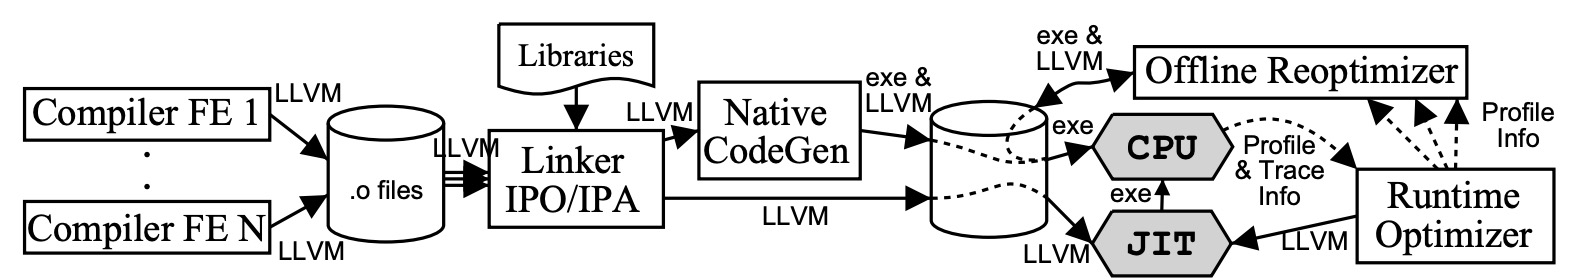
\includegraphics[width=\textwidth]{Imagens/llvm-design.jpg}
    \caption{Diagrama da arquitetura do sistema da LLVM}
    \small{Fonte: \citeonline{lattner2004llvm}}
    \label{fig:llvm-design}
\end{figure}

\citeonline{lattner2004llvm} também argumentam que a arquitetura projetada para a LLVM provê estas cinco capacidades que, em conjunto, a diferencia das demais soluções: (1) modelo de compilação contínua, (2) geração de código \emph{offline}, (3) perfilagem (\emph{profilling}) e otimizações baseadas no usuário, (4) modelo de \emph{runtime} transparente, e (5) compilação uniforme de todo o programa. 

% Compiladores tradicionais oferecem geração de código offline e modelo de tempo de execução transparente, mas carecem de compilação contínua, perfilagem baseada no usuário e compilação de todo o programa. Alguns compiladores comerciais exportam representações intermediárias para otimização em \emph{link-time}, mas não suportam otimização em tempo de execução ou \emph{offline}. Máquinas virtuais de alto nível, como a JVM (Java Virtual Machine), fornecem perfilagem baseada no usuário e compilação contínua parcial, mas faltam geração de código \emph{offline} e modelo de \emph{runtime} transparente. Otimizadores de tempo de execução binário transparentes, como o Dynamo, oferecem geração de código \emph{offline}, modelo de tempo de execução transparente e compilação de todo o programa, mas são limitados na capacidade de otimização devido ao foco em código binário nativo. A Otimização Guiada por Perfil (PGO) para linguagens estáticas oferece perfilagem baseada no usuário, mas não é transparente e pode levar a desempenho sub-ótimo se o treinamento não refletir os padrões de uso reais.

Conforme anteriormente citado, a parte que fundamenta e integra todos os módulos e funcionalidades da LLVM é a sua representação intermediária, a LLVM-IR, que será melhor detalhada na próxima seção.

\subsection{LLVM-IR}\label{sec:llvm-ir}

A representação intermediária de código definida pela LLVM (fundamentada no modelo SSA), traz algumas funcionalidades inovadoras, e serve como uma forma unificada de representar código para fins de análise, modificação e distribuição durante todo o processo de transformação de código \cite{lattner2004llvm}. A especificação de tal representação consiste em um conjunto de instruções similares a de um processador do tipo RISC (do inglês, \emph{Reduced Instruction Set Computer}), mas com informações de alto nível importantes para análises eficazes do código a ser gerado. \citeonline{lattner2004llvm} colocam três principais aspectos:

\begin{enumerate}
    \item[(a)] Um sistema de tipos de baixo nível que pode ser usado para implementar tipos de dados e operações das linguagens de alto nível, expondo os comportamentos implementados a todas as etapas de otimização. Este sistema de tipos inclui informações de tipo que poderão ser usadas por técnicas sofisticadas (independentes de linguagem), como algoritmos para análise de ponteiros, análise de dependências e transformações de dados.
    \item[(b)] Instruções para fazer conversão dos tipos e aritmética de endereços de baixo nível, preservando a informação de tipagem.
    \item[(c)] Duas instruções para tratamento de exceções em baixo nível para implementação de semânticas de exceção específicas das linguagens, mantendo explícito o fluxo de controle ao compilador. 
\end{enumerate}

Quanto à estrutura do código, na representação intermediária da LLVM o fluxo de controle fica explícito, uma vez que "uma função é um conjunto de blocos básicos, e cada bloco básico é uma sequência de instruções LLVM, terminando em exatamente uma instrução terminadora [...]. Cada terminador especifica explicitamente seus blocos básicos sucessores." \cite{lattner2004llvm}.

Segundo a referência da linguagem, o conjunto de instruções da LLVM-IR conta atualmente com mais de 60 códigos de operação (\emph{opcodes}). Dentre estas estão instruções de operações matemáticas, operações em ponteiros, operadores de comparação, instruções de terminação (\emph{return}, \emph{branch}), e também operações mais específicas da solução da LLVM, como conversão entre tipos com diversas opções. O sistema de tipos da LLVM permite a sobrecarga dos operadores para mais de um tipo, ou seja, a instrução \emph{add} por exemplo pode ser usada tanto para inteiros de qualquer tamanho, quanto para ponto flutuantes \cite{llvmLangRef}.

Uma funcionalidade importante do sistema da LLVM, apesar de não visada diretamente nesse trabalho, é o sistema de tipos da LLVM-IR, que conta com diversos tipos nativos, uma robusta instrumentação para definição de tipos compostos, e que é independente da linguagem fonte. Na LLVM todas as variáveis e objetos na memória da representação SSA têm um tipo associado, e todas as operações devem se submeter a regras de tipo específicas \cite{lattner2004llvm}. O sistema de tipos compreende tipos como: \emph{void}, booleano, inteiros com ou sem sinal de 8 até 64 bits e ponto flutuante de precisão simples ou dupla. Além disso, a LLVM contém somente 4 tipos derivados: ponteiros, arrays, estruturas e funções \cite{llvmLangRef}.

A seguir há um código em LLVM-IR gerado utilizando o compilador \emph{clang} a partir de um código em C++. O clang foi utilizado pois a ferramenta de linha de comando tem uma opção para emitir código em LLVM-IR. A versão do \emph{clang} utilizada foi a 15.0.0 em um notebook com processador \emph{Apple M1 Pro}. O comando exato para emitir esse código foi: \verb|clang -emit-llvm -S -O1 fact.cpp|, as flags \verb|-emit-llvm -S| servem para que o \emph{clang} dê como saída código em LLVM-IR e a flag \verb|-O1| foi utilizada por dar a saída já com algumas otimizações e já em forma SSA.

\begin{figure}[h]
    \centering
\begin{lstlisting}[language=llvm,style=nasm]
; ModuleID = 'myfib.c'
source_filename = "myfib.c"
target datalayout = "e-m:o-i64:64-i128:128-n32:64-S128"
target triple = "arm64-apple-macosx14.0.0"

; Function Attrs: nofree norecurse nosync nounwind readnone ssp uwtable(sync)
define i32 @fib(i32 noundef %0) local_unnamed_addr #0 {
  %2 = icmp sgt i32 %0, 99
  br i1 %2, label %12, label %3

3:                                                ; preds = %1
  %4 = icmp sgt i32 %0, 0
  br i1 %4, label %5, label %12

5:                                                ; preds = %3, %5
  %6 = phi i32 [ %8, %5 ], [ 0, %3 ]
  %7 = phi i32 [ %10, %5 ], [ 0, %3 ]
  %8 = phi i32 [ %9, %5 ], [ 1, %3 ]
  %9 = add nsw i32 %6, %8
  %10 = add nuw nsw i32 %7, 1
  %11 = icmp eq i32 %10, %0
  br i1 %11, label %12, label %5, !llvm.loop !6

12:                                               ; preds = %5, %3, %1
  %13 = phi i32 [ -1, %1 ], [ 0, %3 ], [ %8, %5 ]
  ret i32 %13
}

attributes #0 = { nofree norecurse nosync nounwind readnone } ; ...

!llvm.module.flags = !{!0, !1, !2, !3, !4}
!llvm.ident = !{!5}

!0 = !{i32 2, !"SDK Version", [2 x i32] [i32 14, i32 4]}
!1 = !{i32 1, !"wchar_size", i32 4}
; ... continua com mais metadados
\end{lstlisting}                                         
    \caption{Exemplo de Código em LLVM-IR}
    \label{fig:exemplo-llvm-ir}
    \small{Fonte: O autor, gerado usando \emph{clang} e editado}
\end{figure}

Trazendo uma visão geral sobre o código da Figura \ref{fig:exemplo-llvm-ir}: no começo do código há metadados quanto ao arquivo de origem e à arquitetura alvo; linhas iniciadas em ";"\ são comentários; na definição da função, além dos tipos que são obrigatórios, há algumas \emph{flags} para otimização; dentro dos colchetes estão os blocos da forma SSA, o primeiro bloco não necessita explicitamente de um \emph{label}, mas recebe implicitamente o próximo registrador do SSA disponível (nesse caso o "\%1", já que o argumento usa o "\%0"). Também é interessante notar as operações \verb|phi| e \verb|br| (\emph{branch}) e seus argumentos e que todas as operações e instruções carregam tipagem explícita.

A LLVM-IR ser fundamentada na forma SSA quer dizer que cada registrador virtual (variável) é definido exatamente uma vez e o uso de um registrador deve ser dominado por sua definição \cite{lattner2004llvm}; e a LLVM-IR conta com a instrução \verb|phi| explícita, que corresponde diretamente à função $\phi$ da forma SSA \cite{lattner2004llvm}.
